\section{Strategy}

First, let's remind what are weight sharing and auxiliary losses:
\begin{itemize}
	\item Auxiliary losses allows to promote learning for stacked modules (within an architecture) by attaching a prediction to said module(s). The (auxiliary) prediction(s) lead to auxiliary loss(es) during training, incidentally helping with the vanishing gradient issue. The back-propagation is generally done on a weighted sum of the losses. Here, because the information of each channel's digit is known, it is possible to compute a loss on each channel's digit classification in addition to the target classification.
	\item Weight sharing refers to architectures where the same layer(s) are used several times within the network, either in a circular fashion or in a parallel one. Here, because the input consists of two channels of a 14x14 greyscale image representing a digit, each channel can be subjected to the same processing (up until where digit classification happens in case of auxiliary losses use). Thus, up until that moment, the same layers can be used.
\end{itemize}

Because the networks' architectures need to be comparable, it is easier to design the nets in the following order : (1) weight sharing and auxiliary losses (thereafter WS+AL net), (2) weight sharing (thereafter WS net), (3) auxiliary losses (thereafter AL net) and (4) none (thereafter naive net). 

Indeed, it allows to increasingly remove the investigated features from the network as they are designed, thus allowing that the designed layers are adapted to all architectures, while guaranteeing that they remain similar throughout the nets. 

\subsection{Digit classification}
\label{sub::sec::digit_classification}

The network with both weight sharing and auxiliary losses requires a module that can classify a digit, so that module can be shared between both input channels (weight sharing), and so that losses can be computed on it for each input channel (auxiliary losses). 
Thus, the first network implemented is one that classifies the digits.
It was designed with keeping in mind LeNet-5 architecture~\cite{lecun-98}, and illustration on Figure~\ref{fig::dcm} below:

\begin{figure}[H]
	\begin{center}
		\begin{tikzpicture}
		\footnotesize
		\node[anchor=south west,inner sep=0] (image) at (0,0) {\includesvg[width=0.8\textwidth]{dcm}};
		\begin{scope}[x={(image.south east)},y={(image.north west)}]
		
		\node[blue] at (0.045,0.75) {INPUT};
		\node[blue] at (0.965,0.75) {OUTPUT};
		
		\node[] at (0.09, 0) {conv (3,3)};
		\node[align=center] at (0.25, -0.05) {max pool (2,2) \\stride 1 \\padding};
		\node[] at (0.4, 0) {conv (3,3)};
		\node[align=center] at (0.57, -0.15) {max pool (2,2) \\stride 2 \\no padding};
		\node[] at (0.72, 0) {FC};
		\node[] at (0.88, -0.1) {FC};
		\node[] at (0.97, 0.1) {FC};
				
		\end{scope}
		\end{tikzpicture}
		\caption{Digit classification module.}
		\label{fig::dcm}
	\end{center}
\end{figure}

This Digit Classification Module (DCM thereafter) performance was estimated using training and validation sets, both split from an initial training sets, so as to not bias the final accuracy estimation done with testing sets, for any of the networks (since they all use the DCM).
Because the accuracy of this network is found to be is satisfying, it can be used as a module for the WS+AL net. 
Final accuracy estimation (based on testing sets) for all networks is provided later in Section~\ref{sec::results}.

\subsection{Architectures}

From the DCM are then built the other architectures:

\begin{figure}[H]
	\begin{subfigure}[h]{0.495\textwidth}
		\begin{center}
			\begin{tikzpicture}
			\node[anchor=south west,inner sep=0] (image) at (0,0) {\includegraphics[width=0.8\textwidth]{nn_wsal}};
			
			\begin{scope}[x={(image.south east)},y={(image.north west)}]
			
%			\node[] at (0.40, 0.78) {$\theta$};
%			\node[] at (0.7,0.32) {$\theta$};
%			
%			\node[blue] at (0.48,0.98) {$z_1$};
%			\node[blue] at (-0.05,0.2) {$x_1$};
%			\node[blue] at (0.92,0.12) {$y_1$};
%			
%			\node[red] at (0.28,1.04) {$z_2$};
%			\node[red] at (0.06,0.12) {$x_2$};
%			\node[red] at (0.92,0.36) {$y_2$};
			
			\end{scope}
			\end{tikzpicture}
			\caption{WS+AL net}
		\end{center}
	\end{subfigure}
	\begin{subfigure}[h]{0.495\textwidth}
		\begin{center}
			\begin{tikzpicture}
			\node[anchor=south west,inner sep=0] (image) at (0,0) {\includegraphics[width=0.8\textwidth]{nn_al}};
			
			\begin{scope}[x={(image.south east)},y={(image.north west)}]
			
			\end{scope}
			\end{tikzpicture}
			\caption{AL net}
		\end{center}
	\end{subfigure}
	\begin{subfigure}[h]{0.495\textwidth}
		\begin{center}
			\begin{tikzpicture}
			\node[anchor=south west,inner sep=0] (image) at (0,0) {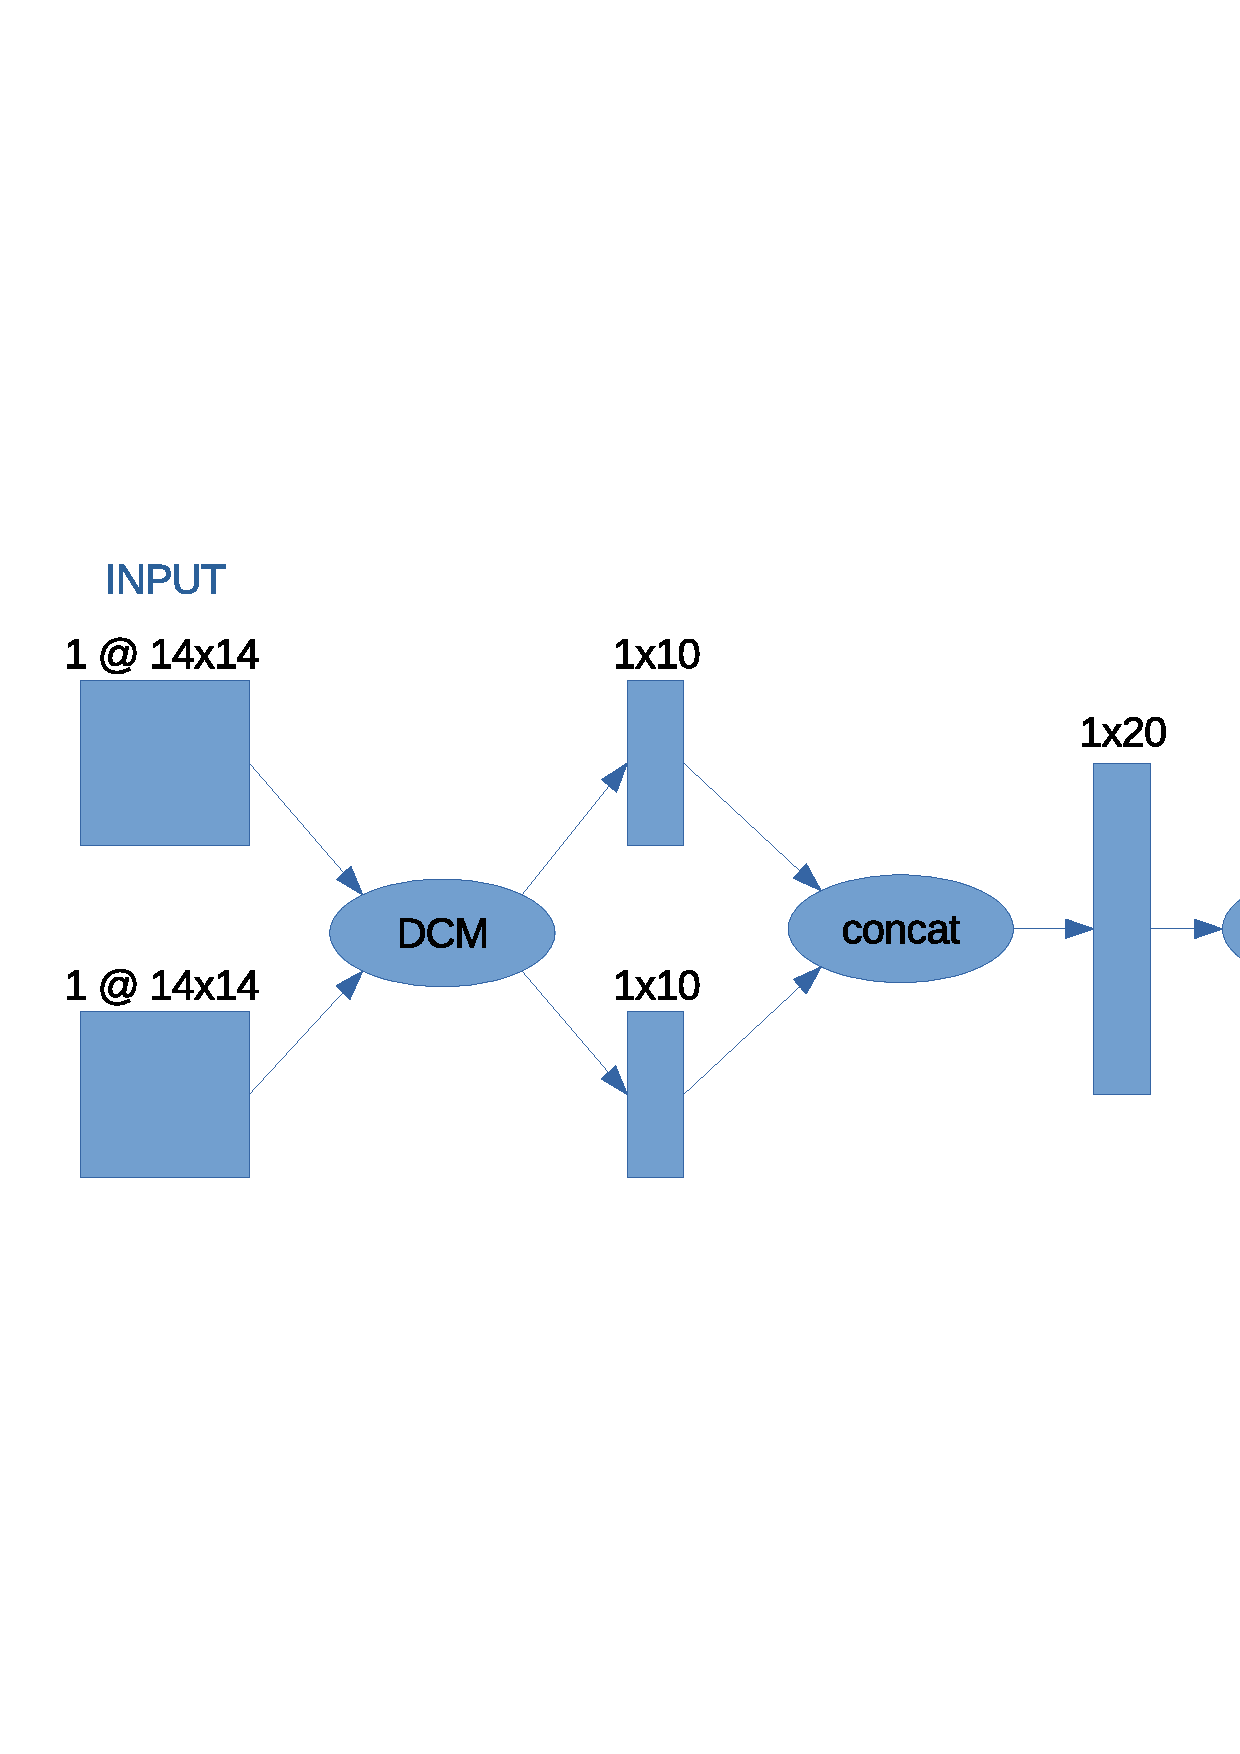
\includegraphics[width=0.8\textwidth]{nn_ws}};
			
			\begin{scope}[x={(image.south east)},y={(image.north west)}]
			
			\end{scope}
			\end{tikzpicture}
			\caption{WS net}
		\end{center}
	\end{subfigure}
	\begin{subfigure}[h]{0.495\textwidth}
	\begin{center}
		\begin{tikzpicture}
			\node[anchor=south west,inner sep=0] (image) at (0,0) {\includegraphics[width=0.8\textwidth]{nn_naive}};
		
		\begin{scope}[x={(image.south east)},y={(image.north west)}]
		
		\end{scope}
		\end{tikzpicture}
		\caption{naive net}
	\end{center}
\end{subfigure}
\caption{Design of the four architectures to be compared.}
\end{figure}

As can be seen, the naive net is not entirely naive, because there is one DCM per input channel (the convolutions don't cross between the two input channels). 
It allows for relevant comparison of the four architectures, which is paramount.


\subsection{Activation functions, criterions and optimizers}

All activation functions are CELUs: 
$\textrm{CELU}(x,\alpha=1) = \max(0,x)+\min \left( 0, \alpha \left( \exp (x/\alpha)-1 \right) \right)$. 
The pros of a CELU are that it is continuously differentiable one time and is evaluated to 0 in 0. 

The criterions are all the cross-entropy loss, as they combine both the negative log likelihood loss and the log softmax.

The optimizers used are all Adams, for an adaptive learning rate.

\subsection{Number of epochs}
\label{sub::sec::number_of_epochs}

The number of epochs on which a network is trained is a pretty big deal. 
If too low, the trained network is underfit, and has lower accuracy than it could have. 
If too high, the trained network is overfit, and cannot generalizes well beyond the training set. 
The trick to estimate a good number of epoch, is to use a training set, a validation set and a testing set. 
The network is trained on the training set. 
At each epoch, the network's accuracy is estimated on the validation set. 
When the accuracy repetitively stops increasing over the epochs on the validation set, overfitting has been reached. 
A previous state of training is kept and tested on the testing set, so as to get unbiased accuracy estimator afterwards.

Here, because the project's guidelines specifically ask that <<all the experiments should be done with 1000 pairs for training and test>>, an optimal number of epochs is estimated by running 20 rounds (let's keep in mind that this is not the optimal number of epochs, but an estimation of it). 
For each round, a set of 1000 pairs are separated into a training set (800 pairs) and a validation set (200 pairs), and the optimal number of epochs is estimated off of it, then averaged. 
With that average estimated optimal number of epochs, the networks are trained with training sets of 1000 pairs, and later tested with testing sets of 1000 pairs (both over 20 rounds as well).
This allows for statistical soundness both for the estimation of the optimal number of epochs, as well as the networks unbiased accuracy estimation.
